\chapter{XỬ LÝ DỮ LIỆU TỪ MPU6050 VÀ ƯỚC LƯỢNG GÓC BẰNG KALMAN FILTER}
\label{chap:mpu-kalman}

% =========================================================
% VAI TRÒ CỦA MPU6050
% =========================================================

\section{Vai trò của MPU6050 trong hệ thống}
\label{sec:mpu-role}

\begin{figure}[H]
    \centering
    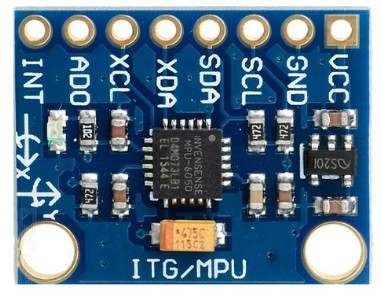
\includegraphics[width=0.55\textwidth]{imgs/mpu6050.jpg}
    \caption{Cảm biến MPU6050}
    \label{fig:mpu6050}
\end{figure}

\setlength{\parindent}{1.25cm}
\setlength{\parskip}{0.3em}

Trong hệ thống điều khiển robot bằng chuyển động nghiêng, cần xác định được hướng và mức độ nghiêng của thiết bị điều khiển để chuyển đổi thành lệnh di chuyển cho robot. Để thực hiện nhiệm vụ này, hệ thống sử dụng cảm biến quán tính MPU6050 \cite{mpu6050-datasheet}.

MPU6050 tích hợp hai loại cảm biến gồm accelerometer ba trục và gyroscope
ba trục. Accelerometer cung cấp thông tin về gia tốc theo ba trục không gian, trong khi gyroscope cung cấp thông tin về vận tốc góc. Hai nguồn dữ liệu này được sử dụng kết hợp để ước lượng góc nghiêng của thiết bị theo hai hướng chính là Pitch và Roll.

Trong hệ thống, MPU6050 giao tiếp với vi điều khiển STM32F103C8T6 thông qua giao thức I2C. Dữ liệu thu được từ cảm biến được xử lý trước khi đưa vào bộ lọc Kalman. Giá trị góc sau khi lọc được sử dụng làm thông tin đầu vào cho khối điều khiển robot.

Quá trình xử lý tổng quát được mô tả như sau:

\begin{figure}[H]
    \centering
    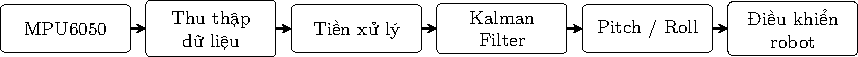
\includegraphics[width=\textwidth]{tikz/processing_flow.pdf}
    \caption{Quá trình xử lý dữ liệu trong hệ thống}
    \label{fig:processing-flow}
\end{figure}

% =========================================================
% NGUYÊN LÝ ĐO ACCELEROMETER VÀ GYROSCOPE
% =========================================================

\section{Nguyên lý đo của Accelerometer và Gyroscope}
\label{sec:sensor-principle}

\subsection{Accelerometer}

Accelerometer được sử dụng để đo gia tốc theo ba trục:

\begin{equation}
A_x,\qquad A_y,\qquad A_z
\end{equation}

Khi cảm biến đứng yên hoặc chuyển động với gia tốc động nhỏ, thành phần gia tốc quan sát được chủ yếu là gia tốc trọng trường. Do hướng của trọng lực tương đối ổn định so với hệ quy chiếu Trái Đất, các thành phần của vector gia tốc trên ba trục có thể được sử dụng để ước lượng góc nghiêng của cảm biến.

MPU6050 hỗ trợ nhiều mức thang đo cho accelerometer \cite{mpu6050-datasheet}, bao gồm:

\begin{table}[H]
\centering
\renewcommand{\arraystretch}{1.3}
\begin{tabular}{|c|c|}
\hline
\textbf{Phạm vi đo} & \textbf{Độ nhạy} \\ \hline
$\pm 2g$  & $16384\ \text{LSB}/g$ \\ \hline
$\pm 4g$  & $8192\ \text{LSB}/g$ \\ \hline
$\pm 8g$  & $4096\ \text{LSB}/g$ \\ \hline
$\pm 16g$ & $2048\ \text{LSB}/g$ \\ \hline
\end{tabular}
\caption{Độ nhạy của cảm biến gia tốc MPU6050}
\label{tab:mpu6050_accel_sensitivity}
\end{table}

Trong hệ thống này, accelerometer được cấu hình ở thang đo:

\begin{equation}
\pm \qty{2}{\g}
\end{equation}

với độ nhạy:

\begin{equation}
\qty{16384}{LSB/\g}
\end{equation}

Do đó, các giá trị gia tốc theo đơn vị $g$ được xác định từ dữ liệu
thô theo:

\begin{equation}
A_x = \frac{A_{x,\text{raw}}}{16384}
\end{equation}

\begin{equation}
A_y = \frac{A_{y,\text{raw}}}{16384}
\end{equation}

\begin{equation}
A_z = \frac{A_{z,\text{raw}}}{16384}
\end{equation}

Ưu điểm của accelerometer là có thể cung cấp thông tin tham chiếu về góc nghiêng trong thời gian dài mà không cần thực hiện phép tích phân vận tốc góc. Tuy nhiên, phép đo của accelerometer dễ bị ảnh hưởng bởi rung động và gia tốc tuyến tính khi thiết bị chuyển động.

Đối với một hệ thống robot, hạn chế này đặc biệt đáng chú ý bởi robot có thể thường xuyên tăng tốc, giảm tốc hoặc thay đổi hướng chuyển động.

\subsection{Gyroscope}

Gyroscope đo vận tốc góc theo ba trục:

\begin{equation}
\omega_x,\qquad \omega_y,\qquad \omega_z
\end{equation}

Trong hệ thống, gyroscope có thể được cấu hình ở nhiều mức thang đo khác nhau \cite{mpu6050-register}, bao gồm:

\begin{table}[H]
\centering
\renewcommand{\arraystretch}{1.3}
\label{tab:gyro_sensitivity}
\begin{tabular}{|c|c|}
\hline
\textbf{Phạm vi đo} & \textbf{Độ nhạy} \\ \hline
$\pm 250\,^\circ/\text{s}$  & $131\,\text{LSB}/(^{\circ}/\text{s})$ \\ \hline
$\pm 500\,^\circ/\text{s}$  & $65.5\,\text{LSB}/(^{\circ}/\text{s})$ \\ \hline
$\pm 1000\,^\circ/\text{s}$ & $32.8\,\text{LSB}/(^{\circ}/\text{s})$ \\ \hline
$\pm 2000\,^\circ/\text{s}$ & $16.4\,\text{LSB}/(^{\circ}/\text{s})$ \\ \hline
\end{tabular}
\caption{Độ nhạy của Gyroscope theo phạm vi đo}
\end{table}

Trong hệ thống này, gyroscope được cấu hình ở mức:

\begin{equation}
\pm 250^\circ/\text{s}
\end{equation}

với độ nhạy:

\begin{equation}
\qty{131}{LSB/(\degree/\second)}
\end{equation}

Mức $\pm 250^\circ/\text{s}$ được lựa chọn vì hệ thống chủ yếu cần theo dõi sự thay đổi góc nghiêng của thiết bị điều khiển, không yêu cầu đo các chuyển động quay có vận tốc góc quá lớn. Việc sử dụng thang đo nhỏ giúp tăng độ nhạy của phép đo trong phạm vi hoạt động của hệ thống.

Vận tốc góc được chuyển đổi từ giá trị raw theo:

\begin{equation}
\omega_x =
\frac{\omega_{x,\text{raw}}}{131}
\end{equation}

\begin{equation}
\omega_y =
\frac{\omega_{y,\text{raw}}}{131}
\end{equation}

\begin{equation}
\omega_z =
\frac{\omega_{z,\text{raw}}}{131}
\end{equation}

Nếu muốn xác định góc từ gyroscope, cần tích phân vận tốc góc theo thời gian:

\begin{equation}
\theta_k =
\theta_{k-1} +
\omega_k \Delta t
\end{equation}

Phương pháp này cho phép gyroscope phản ứng nhanh đối với chuyển động. Tuy nhiên, do tồn tại sai số bias, sai số góc sẽ tích lũy theo thời gian. Giả sử
\begin{equation}
\omega_{\text{measured}}
=
\omega_{\text{true}} + b
\end{equation}
trong đó $b$ là bias của gyroscope. Khi thực hiện tích phân

\begin{equation}
\theta(t)
=
\int
\omega_{\text{measured}}(t)\,dt
\end{equation}
ta có
\begin{equation}
\theta(t)
=
\int \omega_{\text{true}}(t)\,dt
+
\int b(t)\,dt
\end{equation}
Nếu $b \neq 0$, sai số sẽ tăng dần theo thời gian. Hiện tượng này được gọi là \textit{drift}.

% =========================================================
% TÍNH PITCH ROLL
% =========================================================

\section{Tính toán góc Pitch và Roll từ MPU6050}
\label{sec:pitch-roll}

Dữ liệu accelerometer có thể được sử dụng để ước lượng góc nghiêng dựa trên hướng của vector trọng lực.

Đối với góc Roll, hệ thống sử dụng:

\begin{equation}
\phi_{\text{acc}}
=
\operatorname{atan2}(A_y,A_z)
\end{equation}
Sau khi chuyển sang đơn vị độ:
\begin{equation}
\phi_{\text{acc}}
=
\operatorname{atan2}(A_y,A_z)
\frac{180}{\pi}
\end{equation}

Đối với góc Pitch:
\begin{equation}
\theta_{\text{acc}}
=
\operatorname{atan2}
\left(
-A_x,
\sqrt{A_y^2 + A_z^2}
\right)
\end{equation}
hay:
\begin{equation}
\theta_{\text{acc}}
=
\operatorname{atan2}
\left(
-A_x,
\sqrt{A_y^2 + A_z^2}
\right)
\frac{180}{\pi}
\end{equation}

Các công thức trên cho phép chuyển đổi thông tin từ vector gia tốc thành góc nghiêng.

Tuy nhiên, góc được tính trực tiếp từ accelerometer không được sử dụng làm giá trị điều khiển cuối cùng. Nguyên nhân là khi thiết bị chuyển động, accelerometer không chỉ đo gia tốc trọng trường mà còn chịu ảnh hưởng bởi gia tốc động và rung động.

Có thể mô tả phép đo tổng quát:
\begin{equation}
\mathbf{a}_{\text{measured}}
=
\mathbf{a}_{\text{gravity}}
+
\mathbf{a}_{\text{motion}}
+
\mathbf{a}_{\text{noise}}
\end{equation}
khi thành phần $\mathbf{a}_{\text{motion}}$ lớn, góc được suy ra từ accelerometer có thể sai lệch đáng kể so với góc thực. Do đó, trong hệ thống, góc accelerometer được sử dụng như một nguồn thông tin hiệu chỉnh cho thuật toán sensor fusion.

% =========================================================
% NHIỄU VÀ DRIFT
% =========================================================

\section{Vấn đề nhiễu và drift}
\label{sec:noise-drift}

Hai cảm biến trong MPU6050 có những đặc tính sai số khác nhau.

\begin{table}[H]
    \centering
    \renewcommand{\arraystretch}{1.3}
    \label{tab:sensor-comparison}
    \begin{tabular}{p{4cm} p{5cm} p{5cm}}
        \toprule
        \textbf{Đặc tính}
        & \textbf{Accelerometer}
        & \textbf{Gyroscope} \\
        \midrule
        Đại lượng đo
        & Gia tốc
        & Vận tốc góc \\

        Ưu điểm
        & Có thể cung cấp tham chiếu góc dài hạn
        & Phản ứng nhanh với chuyển động \\

        Nhược điểm
        & Nhạy với rung động và gia tốc động
        & Có bias và drift \\

        Vai trò trong hệ thống
        & Measurement để hiệu chỉnh
        & Prediction của góc \\
        \bottomrule
    \end{tabular}
    \caption{So sánh đặc tính của accelerometer và gyroscope}
\end{table}

Nếu chỉ sử dụng accelerometer, góc có thể dao động đáng kể khi robot chuyển động. Nếu chỉ sử dụng gyroscope, góc có thể trôi dần theo thời gian.

Do đó, hệ thống cần kết hợp hai nguồn dữ liệu để tận dụng ưu điểm của mỗi cảm biến.


% =========================================================
% LÝ DO SỬ DỤNG KALMAN
% =========================================================

\section{Lý do sử dụng Kalman Filter}
\label{sec:why-kalman}

Để giải quyết hạn chế của từng cảm biến, hệ thống sử dụng Kalman Filter \cite{welch-kalman} để thực hiện sensor fusion giữa accelerometer và gyroscope \cite{kalmanfilter-vn}.

Ý tưởng chính của phương pháp là sử dụng gyroscope để dự đoán sự thay đổi của góc và sử dụng accelerometer để hiệu chỉnh kết quả dự đoán.

Quá trình này được thực hiện lặp lại liên tục:

\[
\boxed{
\text{Dự đoán}
\rightarrow
\text{Cập nhật phép đo}
\rightarrow
\text{Dự đoán}
\rightarrow
\text{Cập nhật phép đo}
\rightarrow \cdots
}
\tag{1.22}
\]

Có thể biểu diễn:

\begin{figure}[H]
\centering
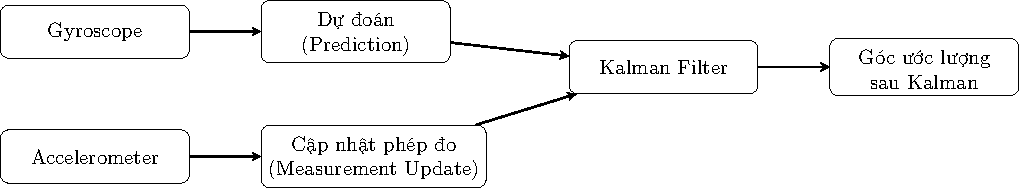
\includegraphics[width=\textwidth]{tikz/kalman_principle.pdf}
\caption{Nguyên lý kết hợp dữ liệu bằng Kalman Filter}
\label{fig:kalman-principle}
\end{figure}

Kalman Filter không đơn giản thực hiện phép trung bình giữa hai phép đo. Thay vào đó, thuật toán sử dụng thông tin về độ không chắc chắn của prediction và measurement để xác định mức độ ảnh hưởng của từng nguồn dữ liệu.

% =========================================================
% CƠ SỞ LÝ THUYẾT
% =========================================================

\section{Cơ sở lý thuyết Kalman Filter}
\label{sec:kalman-theory}

\subsection{Nguyên lý chung}

Kalman Filter là một thuật toán ước lượng trạng thái của một hệ thống từ các phép đo có nhiễu \cite{welch-kalman, lay2021linear}.

Một chu kỳ hoạt động gồm hai bước chính:

\begin{enumerate}
    \item Prediction: dự đoán trạng thái hiện tại từ trạng thái trước đó
    và mô hình chuyển động.
    \item Measurement Update: sử dụng phép đo mới để hiệu chỉnh trạng thái
    dự đoán.
\end{enumerate}

Trong bài toán hiện tại:

\begin{equation}
\text{Gyroscope}
\rightarrow
\text{Prediction}
\end{equation}
và:
\begin{equation}
\text{Accelerometer}
\rightarrow
\text{Measurement}
\end{equation}

\subsection{Mô hình trạng thái}

Đối với mỗi góc, trạng thái được mô hình hóa bởi:

\begin{equation}
\mathbf{x}
=
\begin{bmatrix}
\theta \\
b
\end{bmatrix}
\end{equation}
trong đó:
\begin{itemize}
    \item $\theta$: góc nghiêng ước lượng;
    \item $b$: bias của gyroscope.
\end{itemize}

Như vậy, hệ thống không chỉ ước lượng góc mà còn theo dõi bias của gyroscope trong quá trình hoạt động. Hai bộ lọc độc lập được sử dụng cho Pitch và Roll.

% ---------------------------------------------------------
% PREDICTION
% ---------------------------------------------------------

\subsection{Prediction}

Sau khi loại bỏ bias, vận tốc góc được xác định:
\begin{equation}
\omega_k
=
\omega_{\text{gyro},k}
-
b_{k-1}
\end{equation}

Góc dự đoán:
\begin{equation}
\hat{\theta}_k^{-}
=
\hat{\theta}_{k-1}
+
\omega_k\Delta t
\end{equation}
trong đó:
\begin{itemize}
    \item $\hat{\theta}_{k-1}$ là góc ước lượng tại bước trước;
    \item $\omega_k$ là vận tốc góc đã hiệu chỉnh;
    \item $\Delta t$ là khoảng thời gian giữa hai phép cập nhật;
    \item $\hat{\theta}_k^{-}$ là góc dự đoán trước khi sử dụng measurement.
\end{itemize}

Có thể thấy prediction giúp hệ thống phản ứng nhanh đối với chuyển động, vì thông tin gyroscope được sử dụng trực tiếp để dự đoán thay đổi góc.

% ---------------------------------------------------------
% COVARIANCE
% ---------------------------------------------------------

\subsection{Độ không chắc chắn và ma trận hiệp phương sai}

Ngoài giá trị trạng thái, Kalman Filter còn duy trì ma trận hiệp phương sai:
\begin{equation}
P=
\begin{bmatrix}
P_{00} & P_{01}\\
P_{10} & P_{11}
\end{bmatrix}
\end{equation}

Ma trận $P$ biểu diễn mức độ không chắc chắn của trạng thái ước lượng. Trong quá trình dự đoán, độ không chắc chắn được cập nhật dựa trên:
\begin{itemize}
    \item trạng thái hiệp phương sai hiện tại
    \item khoảng thời gian $\Delta t$
    \item nhiễu quá trình của góc
    \item nhiễu quá trình của bias
\end{itemize}

Sau bước cập nhật phép đo, ma trận hiệp phương sai tiếp tục được cập nhật để phản ánh mức độ chắc chắn mới của trạng thái ước lượng sau khi nhận thêm thông tin từ cảm biến.

% ---------------------------------------------------------
% MEASUREMENT
% ---------------------------------------------------------

\subsection{Measurement Update}

Góc được tính từ accelerometer được xem là measurement:

\begin{equation}
z_k = \theta_{\text{acc}}
\end{equation}

Sai số giữa measurement và prediction được gọi là residual (phần chênh lệch giữa hai giá trị):
\begin{equation}
y_k
=
z_k
-
\hat{\theta}_k^{-}
\end{equation}

Nếu $y_k$ lớn, measurement và prediction đang có sự khác biệt đáng kể.

% ---------------------------------------------------------
% KALMAN GAIN
% ---------------------------------------------------------

\subsection{Kalman Gain}

Kalman Gain là đại lượng quyết định mức độ ảnh hưởng của measurement đến trạng thái ước lượng.

Trong mô hình đơn giản của hệ thống:

\begin{equation}
S=P_{00}+R
\end{equation}

và:

\begin{equation}
K_0=
\frac{P_{00}}{P_{00}+R}
\end{equation}

Trong đó:

\begin{itemize}
    \item $P_{00}$ biểu diễn độ không chắc chắn của góc dự đoán;
    \item $R$ biểu diễn độ không chắc chắn của measurement;
    \item $K_0$ là Kalman Gain của góc.
\end{itemize}

Nếu $R$ lớn, measurement được xem là nhiều nhiễu, do đó Kalman Gain giảm và bộ lọc tin prediction nhiều hơn.

Nếu $R$ nhỏ, measurement được xem là đáng tin cậy hơn, do đó Kalman Gain tăng và measurement có ảnh hưởng lớn hơn.

% ---------------------------------------------------------
% CORRECTION
% ---------------------------------------------------------

\subsection{Hiệu chỉnh trạng thái}

Sau khi tính Kalman Gain, góc được cập nhật:

\begin{equation}
\hat{\theta}_k
=
\hat{\theta}_k^{-}
+
K_0
\left(
z_k-\hat{\theta}_k^{-}
\right)
\end{equation}
hay:
\begin{equation}
\hat{\theta}_k
=
(1-K_0)\hat{\theta}_k^{-}
+
K_0z_k
\end{equation}

Phương trình trên cho thấy kết quả cuối cùng là sự kết hợp giữa prediction và measurement. Khác với phép trung bình thông thường, trọng số của mỗi nguồn dữ liệu được xác định dựa trên độ không chắc chắn của hệ thống.

% ---------------------------------------------------------
% BIAS UPDATE
% ---------------------------------------------------------

\subsection{Cập nhật bias của gyroscope}

Bias được cập nhật dựa trên residual:

\begin{equation}
b_k
=
b_{k-1}
+
K_1y_k
\end{equation}

Nhờ vậy, Kalman Filter có khả năng điều chỉnh ước lượng bias trong quá trình hoạt động thay vì chỉ sử dụng một giá trị cố định. Điều này đặc biệt hữu ích đối với việc hạn chế drift của gyroscope.

% =========================================================
% TRIỂN KHAI
% =========================================================

\section{Triển khai Kalman Filter trong hệ thống}
\label{sec:kalman-implementation}

Trong hệ thống, hai bộ Kalman Filter được sử dụng độc lập để ước lượng Pitch và Roll.

Đối với Pitch:
\begin{equation}
Pitch_{\text{kalman}}
=
Kalman
\left(
Pitch_{\text{acc}},
\omega_y,
\Delta t
\right)
\end{equation}

Đối với Roll:
\begin{equation}
Roll_{\text{kalman}}
=
Kalman
\left(
Roll_{\text{acc}},
\omega_x,
\Delta t
\right)
\end{equation}

Có thể mô tả chuỗi xử lý:
\begin{figure}[H]
    \centering
    \begin{tikzpicture}[
        node distance=0.8cm and 1.2cm,
        box/.style={
            draw,
            rounded corners=2pt,
            minimum height=0.85cm,
            align=center,
            font=\small
        },
        arrow/.style={
            ->,
            >=stealth,
            thick
        }
    ]

    %========================
    % Hàng trên
    %========================
    \node[box, minimum width=3.2cm] (mpu) 
        {MPU6050};

    \node[box, minimum width=3.3cm, below left=1.0cm and 2.5cm of mpu] (acc)
        {Accelerometer\\Đo gia tốc};

    \node[box, minimum width=3.3cm, below right=1.0cm and 2.5cm of mpu] (gyro)
        {Gyroscope\\Đo vận tốc góc};

    %========================
    % Nhánh Accelerometer
    %========================
    \node[box, minimum width=4.2cm, below=0.9cm of acc] (theta)
        {Tính góc từ Accelerometer\\
        $\theta_{acc}$};

    \node[box, minimum width=3.2cm, below=0.9cm of theta] (measurement)
        {Measurement\\Phép đo góc};

    %========================
    % Nhánh Gyroscope
    %========================
    \node[box, minimum width=4.2cm, below=0.9cm of gyro] (bias)
        {Loại bỏ Bias\\
        $\omega = \omega_{gyro} - b$};

    \node[box, minimum width=3.2cm, below=0.9cm of bias] (prediction)
        {Prediction\\Dự đoán góc};

    %========================
    % Kalman Filter - ĐƯA XUỐNG
    %========================
    \node[box, minimum width=3.4cm, below=4.4cm of mpu] (kalman)
        {Kalman Filter};

    \node[box, minimum width=4.2cm, below=0.9cm of kalman] (angle)
        {Góc ước lượng cuối\\Pitch / Roll};

    %========================
    % Mũi tên từ MPU6050
    %========================
    \draw[arrow] (mpu.south west) -- (acc.north);
    \draw[arrow] (mpu.south east) -- (gyro.north);

    %========================
    % Nhánh Accelerometer
    %========================
    \draw[arrow] (acc.south) -- (theta.north);
    \draw[arrow] (theta.south) -- (measurement.north);

    % Measurement -> Kalman
    \draw[arrow] (measurement.east) -- (kalman.west);

    %========================
    % Nhánh Gyroscope
    %========================
    \draw[arrow] (gyro.south) -- (bias.north);
    \draw[arrow] (bias.south) -- (prediction.north);

    % Prediction -> Kalman
    \draw[arrow] (prediction.west) -- (kalman.east);
    
    %========================
    % Kalman -> góc cuối
    %========================
    \draw[arrow] (kalman.south) -- (angle.north);

    \end{tikzpicture}

    \caption{Luồng xử lý dữ liệu MPU6050 và triển khai Kalman Filter}
    \label{fig:mpu6050_kalman}
\end{figure}

Kết quả cuối cùng của bước này là:
\begin{equation}
Pitch_{\text{kalman}}
\end{equation}
và:
\begin{equation}
Roll_{\text{kalman}}
\end{equation}
Đây là hai giá trị góc được sử dụng trong khối điều khiển robot.

% =========================================================
% CALIBRATION
% =========================================================

\section{Calibration MPU6050}
\label{sec:calibration}

Trước khi thực hiện quá trình ước lượng, hệ thống tiến hành calibration để xác định sai số ban đầu của cảm biến.

Trong quá trình calibration, MPU6050 được giữ cố định và hệ thống thu thập nhiều mẫu liên tiếp.

Trong project, tổng cộng 200 mẫu đã được sử dụng.

% ---------------------------------------------------------
% GYRO BIAS
% ---------------------------------------------------------

\subsection{Xác định bias gyroscope}

Bias của gyroscope được tính bằng giá trị trung bình của các phép đo khi cảm biến đứng yên:
\begin{equation}
b_x=
\frac{1}{N}
\sum_{i=1}^{N}
\omega_{x,i}
\end{equation}

Tương tự:
\begin{equation}
b_y=
\frac{1}{N}
\sum_{i=1}^{N}
\omega_{y,i}
\end{equation}

\begin{equation}
b_z=
\frac{1}{N}
\sum_{i=1}^{N}
\omega_{z,i}
\end{equation}

Sau đó, giá trị vận tốc góc được hiệu chỉnh:
\begin{equation}
\omega_{\text{corrected}}
=
\omega_{\text{measured}}
-
b
\end{equation}

Mục đích của bước này là giảm sai số cố định của gyroscope trước khi đưa dữ liệu vào quá trình prediction.

% ---------------------------------------------------------
% ANGLE OFFSET
% ---------------------------------------------------------

\subsection{Xác định Pitch và Roll offset}

Bên cạnh bias của gyroscope, hệ thống cũng xác định góc Pitch và Roll tại tư thế ban đầu.

Các giá trị này được xem như offset:
\begin{equation}
Pitch_{\text{offset}}
\end{equation}
\begin{equation}
Roll_{\text{offset}}
\end{equation}

Góc sau calibration được xác định:
\begin{equation}
Pitch_{\text{cal}}
=
Pitch_{\text{acc}}
-
Pitch_{\text{offset}}
\end{equation}
\begin{equation}
Roll_{\text{cal}}
=
Roll_{\text{acc}}
-
Roll_{\text{offset}}
\end{equation}

Nhờ đó, tư thế ban đầu của thiết bị được quy ước là:
\begin{equation}
Pitch\approx0^\circ
\end{equation}
\begin{equation}
Roll\approx0^\circ
\end{equation}

Điều kiện quan trọng của quá trình calibration là MPU6050 phải được giữ ổn định trong suốt thời gian lấy mẫu.

% =========================================================
% THAM SỐ KALMAN
% =========================================================

\section{Lựa chọn các tham số của Kalman Filter}
\label{sec:kalman-parameters}

Trong hệ thống, ba tham số chính của bộ lọc được sử dụng là:

\begin{equation}
Q_{\text{angle}}=0.001
\end{equation}

\begin{equation}
Q_{\text{bias}}=0.003
\end{equation}

\begin{equation}
R_{\text{measure}}=0.03
\end{equation}

\begin{table}[H]
    \centering
    \caption{Các tham số của Kalman Filter}
    \label{tab:kalman-parameters}
    \begin{tabular}{p{4cm} p{3cm} p{7cm}}
        \toprule
        \textbf{Tham số}
        & \textbf{Giá trị}
        & \textbf{Ý nghĩa} \\
        \midrule
        $Q_{\text{angle}}$
        & 0.001
        & Mức độ không chắc chắn của mô hình góc \\

        $Q_{\text{bias}}$
        & 0.003
        & Mức độ biến thiên được giả định của bias gyroscope \\

        $R_{\text{measure}}$
        & 0.03
        & Mức độ nhiễu của measurement từ accelerometer \\
        \bottomrule
    \end{tabular}
\end{table}

Các giá trị này không phải là các giá trị cố định bắt buộc đối với MPU6050 mà là các tham số dùng để điều chỉnh đặc tính của bộ lọc.

\subsection{Ảnh hưởng của \texorpdfstring{$Q_{\text{angle}}$}{Q\_angle}}

Khi tăng $Q_{\text{angle}}$, hệ thống giả định rằng mô hình prediction có nhiều bất định hơn. Do đó, measurement có xu hướng có ảnh hưởng lớn hơn đến kết quả. Ngược lại, khi giảm $Q_{\text{angle}}$, bộ lọc có xu hướng tin prediction nhiều hơn.

\subsection{Ảnh hưởng của \texorpdfstring{$Q_{\text{bias}}$}{Q\_bias}}

Tăng $Q_{\text{bias}}$ cho phép bộ lọc thích nghi nhanh hơn với sự thay đổi của bias gyroscope. Giảm $Q_{\text{bias}}$ khiến bias được xem là ổn định hơn và thay đổi chậm hơn.

\subsection{Ảnh hưởng của \texorpdfstring{$R_{\text{measure}}$}{R\_measure}}

Nếu tăng $R_{\text{measure}}$, measurement từ accelerometer được xem là nhiều nhiễu hơn. Bộ lọc sẽ giảm mức độ tin tưởng vào accelerometer và duy trì nhiều hơn thông tin từ prediction. Nếu giảm $R_{\text{measure}}$, accelerometer được xem là đáng tin cậy hơn và ảnh hưởng mạnh hơn đến kết quả. Do đó, tuning các tham số $Q$ và $R$ cần được thực hiện dựa trên đặc tính thực tế của cảm biến cũng như yêu cầu về độ mượt và tốc độ đáp ứng của  obot.

% =========================================================
% DT
% =========================================================

\section{Tính toán khoảng thời gian \texorpdfstring{$\Delta t$}{Delta t}}
\label{sec:dt}

Kalman Filter cần biết khoảng thời gian giữa hai lần cập nhật liên tiếp để thực hiện bước prediction. Khoảng thời gian này được xác định theo:
\begin{equation}
\Delta t
=
t_k-t_{k-1}
\end{equation}

Trong chương trình, thời điểm thực hiện mỗi lần đọc dữ liệu MPU6050 được xác định dựa trên bộ đếm thời gian của hệ thống. Khoảng thời gian giữa hai lần cập nhật được chuyển đổi từ mili-giây sang giây theo:
\begin{equation}
\Delta t
=
\frac{t_k-t_{k-1}}{1000}
\end{equation}

Giá trị $\Delta t$ được sử dụng trực tiếp trong bước prediction của Kalman Filter:
\begin{equation}
\theta_k^-
=
\theta_{k-1}
+
\omega_k\Delta t
\end{equation}

Do thời gian thực hiện các tác vụ trong vòng lặp có thể thay đổi, $\Delta t$ không được xem là một giá trị cố định mà được tính toán lại ở mỗi chu kỳ xử lý dựa trên thời gian thực tế giữa hai lần cập nhật liên tiếp.

Vòng lặp chính được thiết lập với khoảng thời gian xử lý mục tiêu khoảng $20$ ms. Do đó, tần số xử lý của vòng lặp có thể được ước tính xấp xỉ:
\begin{equation}
f_{\text{loop}}
\approx
\frac{1}{0.02}
= \qty{50}{\hertz}
\end{equation}

Trong khi đó, MPU6050 được cấu hình với tần số lấy mẫu:
\begin{equation}
f_{\text{MPU6050}}=\qty{100}{\hertz}
\end{equation}

Như vậy, cảm biến được cấu hình với tần số lấy mẫu cao hơn tần số xử lý của vòng lặp chính. Trong chương trình hiện tại, dữ liệu cảm biến được đọc và đưa vào Kalman Filter với tần số xử lý mục tiêu khoảng $50$ Hz, trong khi giá trị $\Delta t$ được sử dụng trong bộ lọc vẫn được xác định dựa trên thời gian thực tế giữa hai lần cập nhật.

% =========================================================
% LUỒNG XỬ LÝ
% =========================================================

\section{Luồng xử lý dữ liệu hoàn chỉnh}
\label{sec:complete-flow}

Toàn bộ quá trình xử lý dữ liệu trong hệ thống được thực hiện theo các bước sau.

\subsection{Bước 1: Thu thập dữ liệu}

MPU6050 cung cấp:
\begin{equation}
A_x,\ A_y,\ A_z
\end{equation}
và:
\begin{equation}
\omega_x,\ \omega_y,\ \omega_z
\end{equation}

\subsection{Bước 2: Tiền xử lý và calibration}

Dữ liệu raw được chuyển đổi sang đơn vị vật lý và hiệu chỉnh bias gyroscope cùng với offset góc ban đầu.

\subsection{Bước 3: Tính góc từ accelerometer}

Từ dữ liệu $A_x$, $A_y$ và $A_z$, hệ thống tính:
\begin{equation}
Pitch_{\text{acc}}
\end{equation}
và:
\begin{equation}
Roll_{\text{acc}}
\end{equation}

\subsection{Bước 4: Prediction}

Gyroscope cung cấp vận tốc góc để dự đoán trạng thái tiếp theo.

\subsection{Bước 5: Measurement Update}

Góc từ accelerometer được sử dụng để hiệu chỉnh giá trị dự đoán.

\subsection{Bước 6: Xuất góc sau lọc}

Kết quả cuối cùng là:
\begin{equation}
Pitch_{\text{kalman}}
\end{equation}
và:
\begin{equation}
Roll_{\text{kalman}}
\end{equation}

\subsection{Bước 7: Tạo lệnh điều khiển}

Pitch sau Kalman được sử dụng để xác định mức độ điều khiển tiến/lùi, trong khi Roll được sử dụng để xác định mức độ điều khiển rẽ.

\begin{figure}[H]
    \centering
    \fbox{
        \begin{minipage}{0.90\textwidth}
            \centering

            \textbf{MPU6050}

            $\downarrow$

            Dữ liệu Accelerometer + Gyroscope

            $\downarrow$

            Tiền xử lý + Calibration

            \vspace{0.3cm}

            \begin{tabular}{cc}
                \textbf{Pitch} & \textbf{Roll} \\[2mm]
                Pitch từ Accelerometer & Roll từ Accelerometer \\ 
                Gyroscope Y & Gyroscope X \\[2mm]
                $\downarrow$ & $\downarrow$ \\[1mm]
                Kalman Filter & Kalman Filter \\[1mm]
                $\downarrow$ & $\downarrow$ \\[1mm]
                $Pitch_{\text{kalman}}$ & $Roll_{\text{kalman}}$ \\[2mm]
                $\downarrow$ & $\downarrow$ \\[1mm]
                Forward control & Turn control
            \end{tabular}

            \vspace{0.3cm}

            $\downarrow$

            \textbf{Robot}

        \end{minipage}
    }
    \caption{Luồng xử lý dữ liệu từ MPU6050 đến điều khiển robot}
    \label{fig:complete-flow}
\end{figure}

% =========================================================
% CHUYỂN GÓC THÀNH CONTROL
% =========================================================

\section{Chuyển đổi góc thành tín hiệu điều khiển}
\label{sec:angle-control}

Sau khi có góc Pitch và Roll sau Kalman, hệ thống chuyển đổi chúng thành các giá trị điều khiển.

Khoảng góc hoạt động được giới hạn:
\begin{equation}
-60^\circ \leq \theta \leq +60^\circ
\end{equation}
và được ánh xạ sang:
\begin{equation}
-80 \leq u \leq +80
\end{equation}
trong đó $u$ là giá trị điều khiển (giới hạn ở mức 80\% công suất tối đa để bảo vệ cơ cấu chấp hành).

Hệ thống đồng thời sử dụng vùng chết:
\begin{equation}
-8^\circ < \theta < +8^\circ
\end{equation}
Trong vùng này, tín hiệu điều khiển được đặt bằng 0 nhằm tránh robot phản ứng với các dao động nhỏ của góc.

Mối quan hệ giữa góc và giá trị điều khiển được mô tả bằng hàm phi tuyến bậc hai (Exponential Response), giúp hệ thống tay lái hoạt động mượt mà ở góc nghiêng nhỏ và nhạy ở góc nghiêng lớn:
\begin{equation}
u = \mathrm{sign}(\theta) \times \left( \frac{|\theta| - 8}{60 - 8} \right)^2 \times 80
\end{equation}
với điều kiện:
\begin{equation}
8^\circ \leq |\theta| \leq 60^\circ
\end{equation}

Bảng sau minh họa quá trình ánh xạ mẫu theo công thức trên:
\begin{table}[H]
    \centering
    \renewcommand{\arraystretch}{1.3}
    \caption{Ánh xạ góc nghiêng sang giá trị điều khiển thực tế}
    \label{tab:angle-control}
    \begin{tabular}{c r @{} l}
        \toprule
        \textbf{Góc nghiêng} & \multicolumn{2}{c}{\textbf{Giá trị điều khiển}} \\
        \centering
        $-60^\circ$ & $-$ & $80$ \\
        $-34^\circ$ & $-$ & $20$ \\
        $0^\circ$ & & $0$ \\
        $+34^\circ$ & $+$ & $20$ \\
        $+60^\circ$ & $+$ & $80$ \\
        \bottomrule
    \end{tabular}
\end{table}

Trong hệ thống:
\begin{equation}
control_{\text{forward}}
=
f(Pitch_{\text{kalman}})
\end{equation}
và:
\begin{equation}
control_{\text{turn}}
=
f(Roll_{\text{kalman}})
\end{equation}

Điều này tạo ra mối liên hệ trực tiếp giữa góc nghiêng sau Kalman và giá trị điều khiển tiến/lùi hoặc rẽ của hệ thống.

% =========================================================
% THUẬT NGỮ
% =========================================================

% Các thuật ngữ chuyên ngành đã được gộp chung và định nghĩa tại mục Danh sách các từ viết tắt và thuật ngữ ở phần đầu báo cáo.

